\documentclass{article}
\usepackage{graphicx}
\usepackage[left=3.5cm, right = 3.5cm, top=3.5cm, bottom=3.5cm, head=13.6pt]{geometry}
\usepackage[onehalfspacing]{setspace}
\usepackage{amsthm}
\usepackage{amsmath}
\usepackage{amssymb}
\usepackage{mathtools}
\usepackage{float}
\usepackage{algpseudocode}
\usepackage{algorithm}
\usepackage{comment}
\usepackage{csquotes}
\usepackage{enumitem}


\title{Advanced Topics in Computer Graphics I - Sheet R05}
\author{Ninian Kaspers, Robin Landsgesell, Julian Stamm}
\date{\today}

\begin{document}

    \maketitle

    \section*{Assignment 2}

    a)\\
    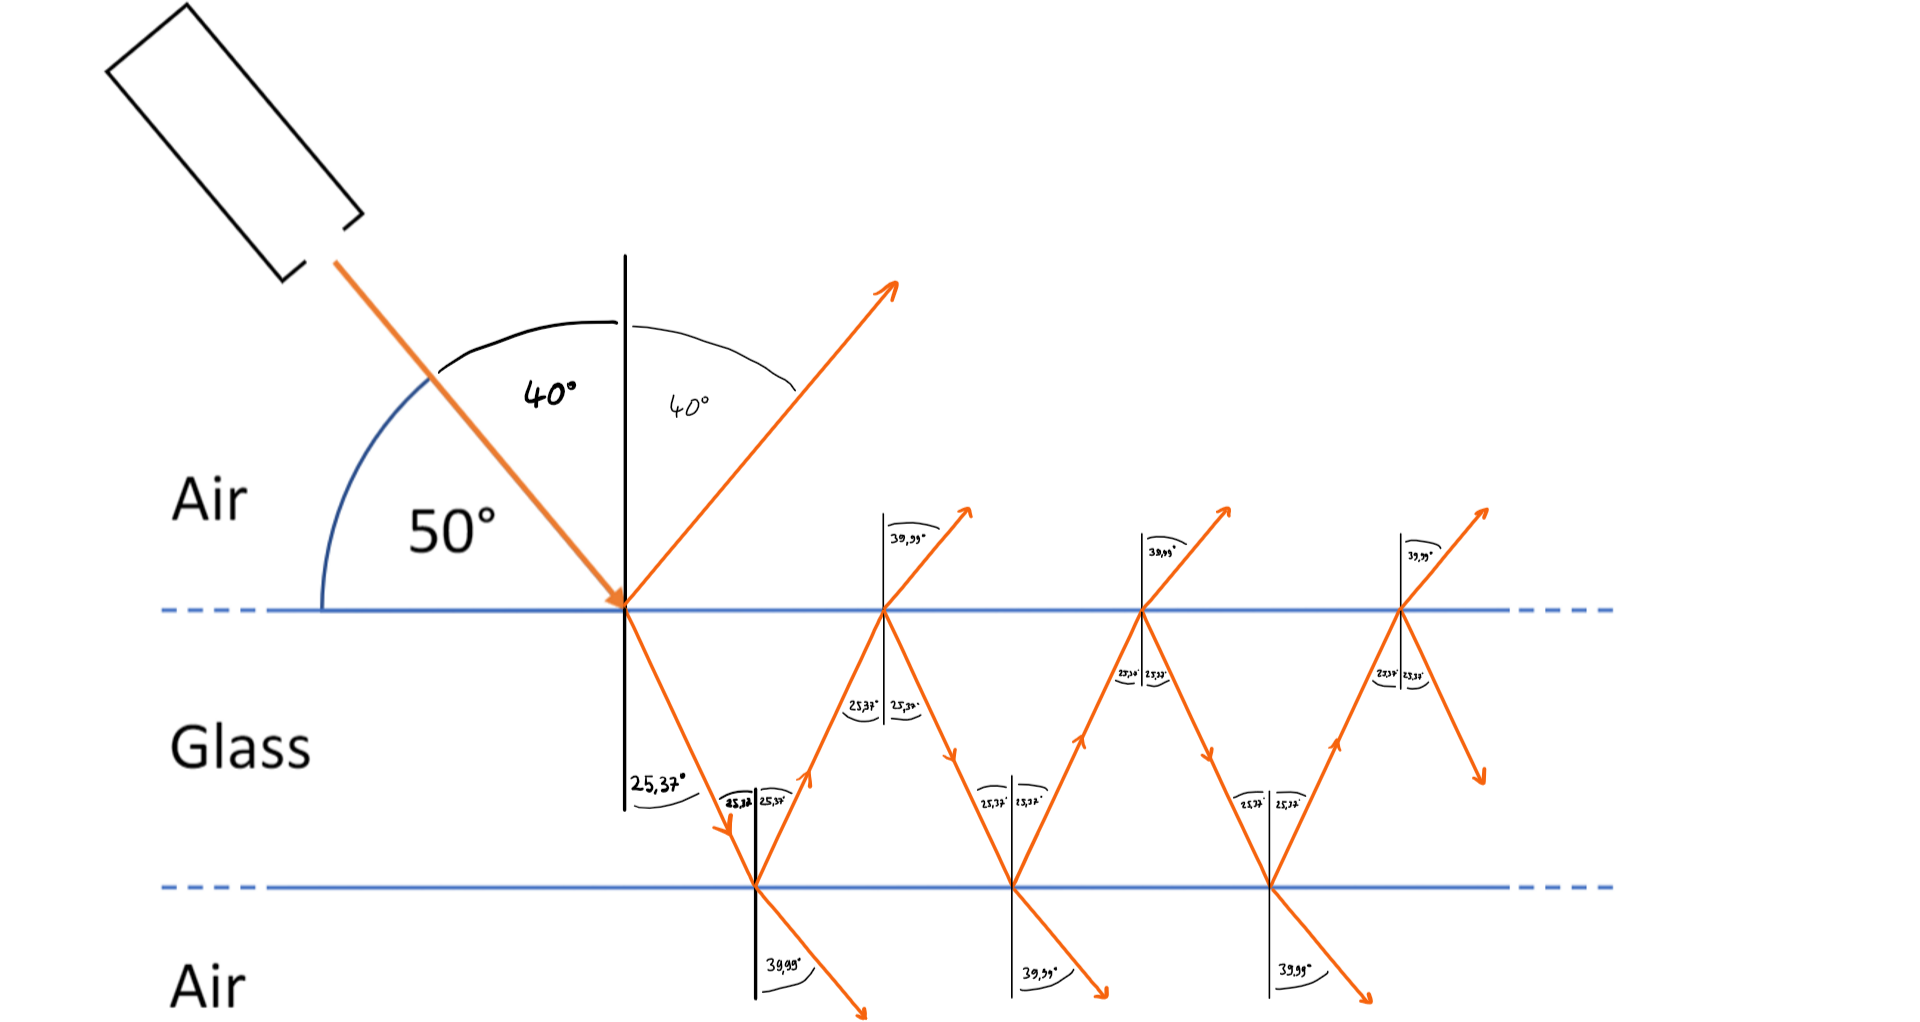
\includegraphics[width=\textwidth]{2a.png}
    \\
    b)\\
    Fresnel equations:\\
    Reflectance for unpolarized light:\\
    \begin{align*}
        R &= \frac{T_\perp^2  + T_\parallel^2}{2} = \frac{\left(\frac{n_i \cos{\theta_i} - n_t \cos{\theta_t}}{n_i \cos{\theta_i} + n_t \cos{\theta_t}}\right)^2 + \left(\frac{n_t \cos{\theta_i} - n_i \cos{\theta_t}}{n_t \cos{\theta_i} + n_i \cos{\theta_t}}\right)^2}{2}\\
        R &\approx \frac{\left(\frac{1 \cdot \cos{40^\circ} - 1.5 \cdot \cos{25.37^\circ}}{1 \cdot \cos{40^\circ} + 1.5 \cdot \cos{25.37^\circ}}\right)^2 + \left(\frac{1.5 \cdot \cos{40^\circ} - 1 \cdot \cos{25.37^\circ}}{1.5 \cdot \cos{40^\circ} + 1 \cdot \cos{25.37^\circ}}\right)^2}{2}\\
        R &\approx 0.0457359
    \end{align*}
    Transmittance:
    \begin{align*}
        T &= 1 - R\\
        T &\approx 0.9542641
    \end{align*}
    For infinite interactions:\\
    Total emission to the top:\\
    \begin{align*}
        &&               R_{\text{total}} &= R + T^2 R \sum_{k=0}^{\infty} (R^2)^k\\
        &\Rightarrow&    R_{\text{total}} &= R + \frac{T^2 R}{1 - R^2}\\
        &&               R_{\text{total}} &\approx 0.0457359 + \frac{0.9542641^2 \cdot 0.0457359}{1 - 0.0457359^2} \approx 0.087471
    \end{align*}
    Total emission to the bottom:\\
    \begin{align*}
        &&               T_{\text{total}} &= T^2 \sum_{k=0}^{\infty} (R^2)^k\\
        &\Rightarrow&    T_{\text{total}} &= \frac{T^2}{1 - R^2}\\
        &&               T_{\text{total}} &\approx \frac{0.9542641^2}{1 - 0.0457359^2} \approx 0.912529
    \end{align*}
    
    \section*{Assignment 3}

    
\end{document}
